\documentclass[conference]{IEEEtran}
\usepackage{graphicx}
\usepackage{amsmath}
\usepackage{booktabs}
\usepackage{xcolor}
\graphicspath{{figures/}}

% Marks text that still has to be filled in from the personal dataset.
\newcommand{\todo}[1]{\textcolor{red}{[TODO: #1]}}

\begin{document}

\title{SudokuScan: From a Photograph of a Printed Puzzle\\to a Digital $9\times 9$ Grid}
\author{\todo{Name Surname, student number}\\COMP 482 Computer Vision, Project 1}
\maketitle

\begin{abstract}
This report describes a pipeline that reads a printed sudoku puzzle from a
phone photograph. The four outer corners of the grid are found with the
Harris detector, the puzzle is rectified with two affine models and a
homography, and the printed digits are read with Tesseract. On the 20
development images the mean corner error is 0.28\,\% of the puzzle side and
all 81 cells are correct in every image. \todo{one sentence with the same
numbers on the personal dataset}. The comparison of the three models shows
that an affine map is only acceptable for near-frontal views.
\end{abstract}

\section{Introduction}
A sheet of paper is a plane, so its image under a pinhole camera is related
to the flat puzzle by a homography. The task is to undo this mapping
automatically and read the 81 cells. The difficulties are (i) finding the
four outer corners among hundreds of corner-like points produced by grid
intersections, digits and surrounding text, (ii) uneven lighting and
(iii) an OCR engine that is designed for lines of text, not single digits.

The pipeline has six stages, each a separate function in
\texttt{sudoku\_scan.py}: preprocessing, Harris corner detection with
automatic corner selection, rectification with three models (A3, A4, H4),
their comparison, cell extraction with digit recognition, and a validity
check. It uses only OpenCV, NumPy and Tesseract, and takes about 3\,s per
image on a CPU.

\section{Corner Detection}
\subsection{Preprocessing}
The image is downscaled so that its longest side is 1000\,px and converted
to grey. All later sizes are fractions of this working size, so a 1000\,px
and a 4000\,px photograph are treated identically; corners are scaled back
to original pixels at the end.

Lighting is normalised by binarisation. After a $3\times3$ Gaussian blur,
the local paper brightness $P$ is estimated with a morphological closing
(kernel 2\,\% of the image width), which removes dark structures thinner
than the kernel, such as lines and digits. A pixel $I$ is ink when
$I < 0.85\,P$. Because the test is a ratio, it gives the same result in a
bright and a dark photograph, which a fixed offset from the local mean
(\texttt{cv2.adaptiveThreshold}) does not.

\subsection{Harris response and candidates}
\texttt{cv2.cornerHarris} is applied to the binary image. The response is
$R=\det M-k\,(\operatorname{trace}M)^2$, where $M$ is the structure tensor
summed over a \texttt{blockSize} neighbourhood of gradients computed with a
Sobel filter of aperture \texttt{ksize}. Working on the binary image gives
every ink edge the same contrast, so a threshold relative to the maximum
response does not discard corners that lie in shadow.

Candidates are pixels with $R > 0.05\,R_{\max}$ that are also local maxima:
a pixel is kept when it equals the grey-scale dilation of $R$ with a window
of 0.5\,\% of the image width. The window must be smaller than the thickness
of the outer border; with a 1\,\% window the outer and inner corner of the
thick border merged into one peak, and the corner error of several images
rose above 1\,\%.

\subsection{Corner selection rule}
\textbf{Region.} In the binary image the sudoku grid is one connected
component with 81 holes. For every component found by
\texttt{cv2.findContours} (\texttt{RETR\_CCOMP}) the holes with an area
between $1/400$ and $1/5$ of the component area are counted. Components that
touch the image border are discarded, since the puzzle is fully visible. The
puzzle is the component whose count is closest to 81. Text and the page edge
have almost no such holes, an empty rectangle has one hole that is too
large, and a crossword has too many.

\textbf{Corners.} Only Harris candidates that lie on this component
(dilated by one pixel) are kept, which removes text printed next to the
grid. The four outer corners are the four points of the convex hull of these
candidates that span the quadrilateral of largest area. They are ordered
TL, TR, BR, BL by their angle around the centroid and refined with
\texttt{cv2.cornerSubPix}. Contours are used only to find the region; all
coordinates come from the Harris detector.

\subsection{Parameter study}
One parameter was varied at a time around the chosen values
(\texttt{blockSize}\,=\,5, \texttt{ksize}\,=\,3, $k$\,=\,0.04,
threshold\,=\,0.05). Table~\ref{tab:params} and Fig.~\ref{fig:params} show
the mean number of candidates and the mean corner error on the 20
development images. \todo{repeat on at least 6 personal images with
\texttt{tools/param\_study.py} and report those numbers}.

\begin{table}[t]
\caption{Harris parameter study (development set, 20 images)}
\label{tab:params}
\centering
\begin{tabular}{llrrr}
\toprule
Parameter & Value & Candidates & Error (\%) & Failures\\
\midrule
blockSize & 2 & 2624 & 0.46 & 0\\
          & 3 & 2462 & 0.28 & 0\\
          & \textbf{5} & 2128 & 0.28 & 0\\
          & 7 & 1859 & 0.28 & 0\\
          & 13 & 2697 & 0.63 & 0\\
ksize     & \textbf{3} & 2128 & 0.28 & 0\\
          & 5 & 1455 & 0.28 & 0\\
          & 7 & 1393 & 0.28 & 0\\
$k$       & 0.02 & 2988 & 0.28 & 0\\
          & \textbf{0.04} & 2128 & 0.28 & 0\\
          & 0.10 & 1558 & 0.28 & 0\\
          & 0.20 & 1221 & 1.24 & 0\\
threshold & 0.01 & 3426 & 0.28 & 0\\
          & \textbf{0.05} & 2128 & 0.28 & 0\\
          & 0.20 & 1276 & 0.30 & 0\\
          & 0.40 & 793 & 4.65 & 8\\
          & 0.60 & 200 & 21.72 & 20\\
\bottomrule
\end{tabular}
\end{table}

\begin{figure*}[t]
\centering
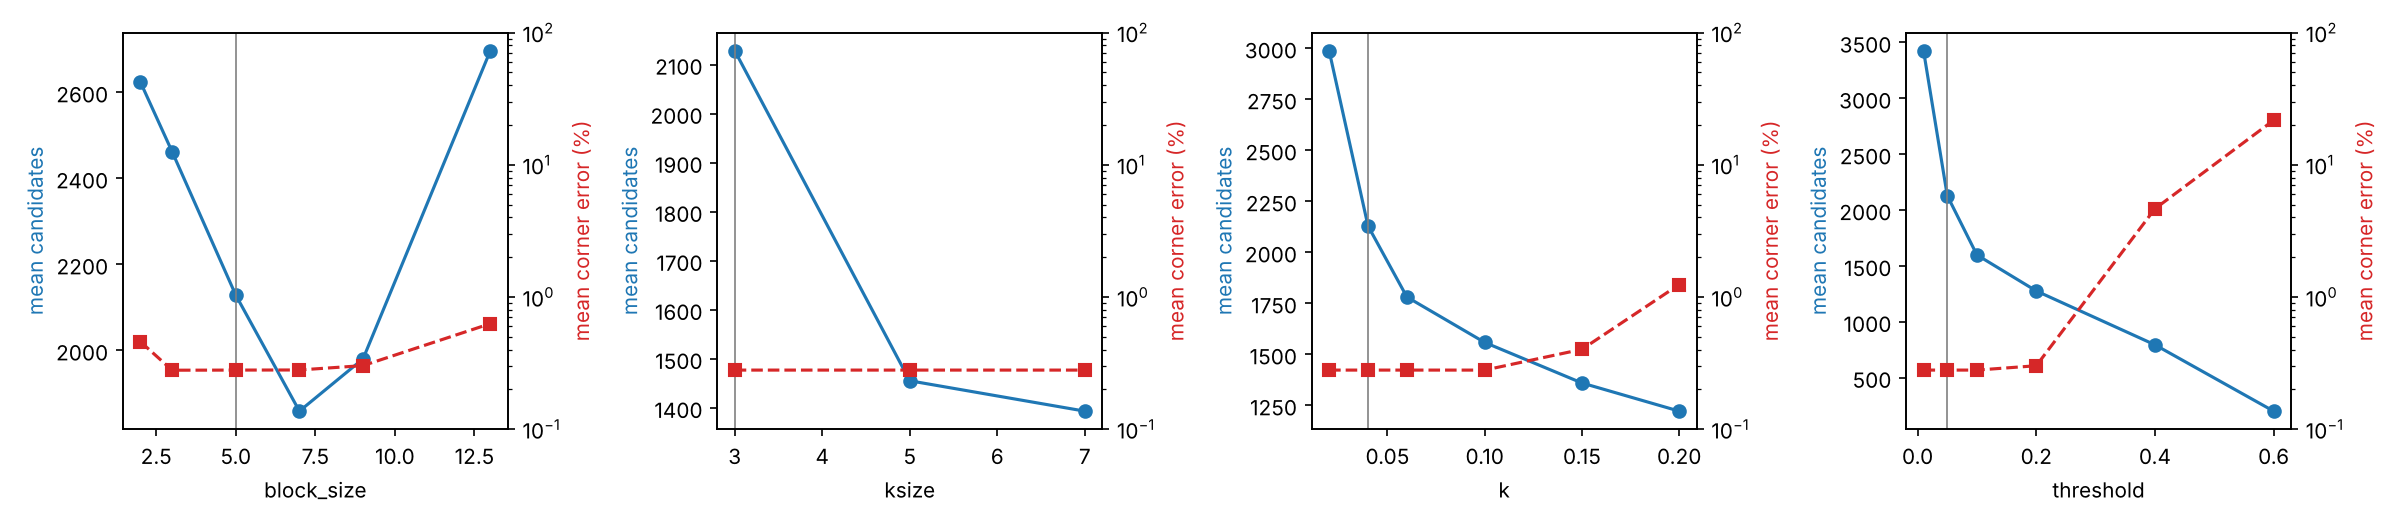
\includegraphics[width=\textwidth]{devset/param_study.png}
\caption{Number of candidates (blue) and corner error (red, log scale) for
each Harris parameter on the development set. The grey line is the chosen
value.}
\label{fig:params}
\end{figure*}

The corner error is flat over a wide range, because the selection rule only
needs the four outer corners to be among the candidates. A small
\texttt{blockSize} (2) gives a noisy response, and a large one (13) blurs it
and shifts the peak away from the true corner. A large $k$ penalises
edge-like structure more strongly and starts to remove the outer corners at
$k = 0.2$. The threshold is the most sensitive parameter: above 0.2 the
outer corners themselves are rejected and the rule fails. The chosen values
lie in the middle of the flat range; the low threshold keeps a safety margin
for photographs with weaker corners.

\subsection{Cases the rule fails on}
The rule assumes that the grid is one connected component with closed cells
and that nothing else is attached to it. It fails when an object or text
touches the outer border in the binary image, when the grid lines are too
faint to close the cells, and when the puzzle is cut by the image border.
\todo{add the failures observed on the personal dataset}.

\section{Rectification}
The four corners are mapped to a $450\times450$ square (50\,px per cell)
with three models.

\textbf{A3} (\texttt{cv2.getAffineTransform}) is the affine map through TL,
TR and BL. An affine map
$\mathbf{x}' = A\mathbf{x} + \mathbf{t}$ has six parameters and every point
pair gives two equations, so three pairs determine it exactly. The fourth
corner is not used; where it lands measures how far the view is from affine.

\textbf{A4} (\texttt{cv2.estimateAffine2D}) is the least-squares affine fit
to all four corners. With the reprojection threshold set to the image size
all four points are inliers, so the result equals the ordinary least-squares
solution. It spreads the error over the four corners; the RMS residual is
reported.

\textbf{H4} (\texttt{cv2.getPerspectiveTransform}) is the homography through
all four corners. A homography is a $3\times3$ matrix defined up to scale,
so it has eight degrees of freedom and needs four point pairs. The two
additional parameters form the last row and make the denominator depend on
the position, which models perspective foreshortening.

An affine map preserves parallelism: it turns a square into a parallelogram
and can model rotation, scale and shear but no vanishing point. A homography
maps lines to lines without preserving parallelism, so it can represent any
view of a plane. On the development set H4 maps the four corners onto the
target square with a maximum error below $10^{-4}$\,px, while the A3
fourth-corner error ranges from 16 to 262\,px and the A4 RMS residual from 4
to 55\,px.

\section{Affine versus Homography}
\textbf{Obliqueness.} Obliqueness is defined as the largest ratio between
the lengths of opposite sides of the detected quadrilateral. It is exactly 1
for every parallelogram, so it ignores in-plane rotation and measures only
the perspective part of the distortion.

\textbf{Measures.} (1) The A3 fourth-corner error and the A4 RMS residual.
(2) Grid line deviation: the rectified image is binarised and projected onto
each axis; near each of the 20 ideal line positions (every 50\,px) the
strongest peak of the profile is located, and the mean distance to the ideal
position is reported. (3) Cell accuracy of the same recognition stage on
each rectification.

\textbf{Results.} Fig.~\ref{fig:models} shows the three measures on the
development set and Table~\ref{tab:models} summarises them.
\todo{replace or complement with the personal dataset (at least 8 images):
run \texttt{tools/compare\_models.py}, include
\texttt{personal/model\_comparison.png} and \texttt{personal/most\_oblique.png}.}

\begin{figure*}[t]
\centering
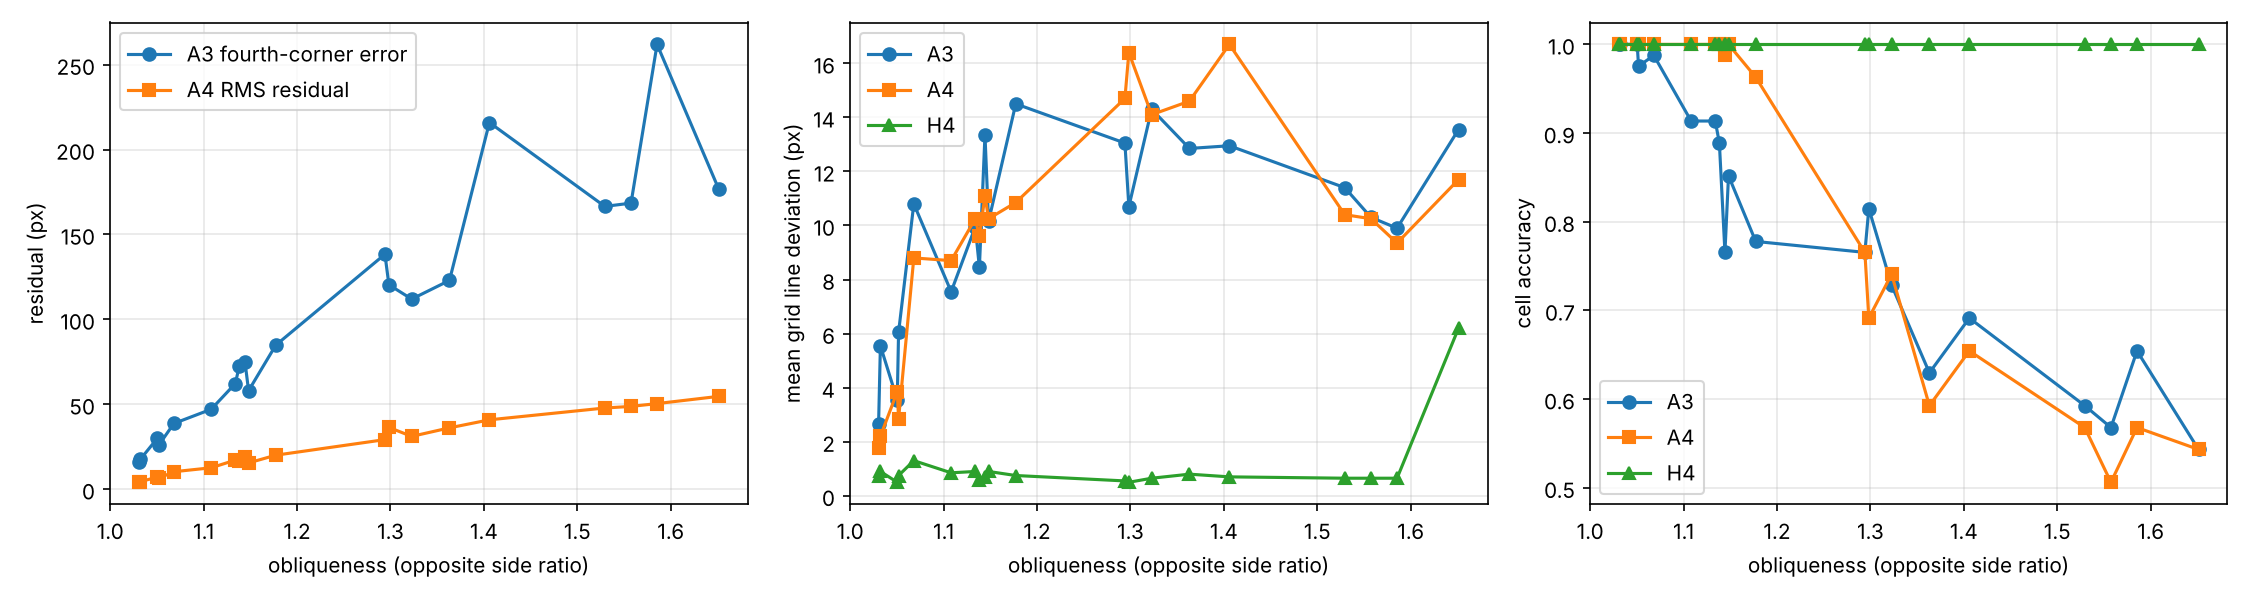
\includegraphics[width=\textwidth]{devset/model_comparison.png}
\caption{Corner residuals, grid line deviation and cell accuracy against
obliqueness (development set).}
\label{fig:models}
\end{figure*}

\begin{table}[t]
\caption{Affine versus homography by obliqueness (development set)}
\label{tab:models}
\centering
\begin{tabular}{lrrr}
\toprule
Obliqueness & $\le 1.07$ & 1.10--1.18 & $\ge 1.29$\\
Images & 5 & 6 & 9\\
\midrule
A3 error (px) & 16--39 & 47--85 & 112--262\\
A4 RMS (px) & 4--10 & 13--20 & 29--55\\
Line dev.\ A3 (px) & 2.7--10.8 & 7.6--14.5 & 9.9--14.3\\
Line dev.\ A4 (px) & 1.8--8.8 & 8.7--11.1 & 9.4--16.7\\
Line dev.\ H4 (px) & 0.5--1.3 & 0.6--0.9 & 0.5--6.2\\
Cell acc.\ A3 & 0.98--1.00 & 0.77--0.91 & 0.54--0.82\\
Cell acc.\ A4 & 1.00 & 0.96--1.00 & 0.51--0.77\\
Cell acc.\ H4 & 1.00 & 1.00 & 1.00\\
\bottomrule
\end{tabular}
\end{table}

\begin{figure}[t]
\centering
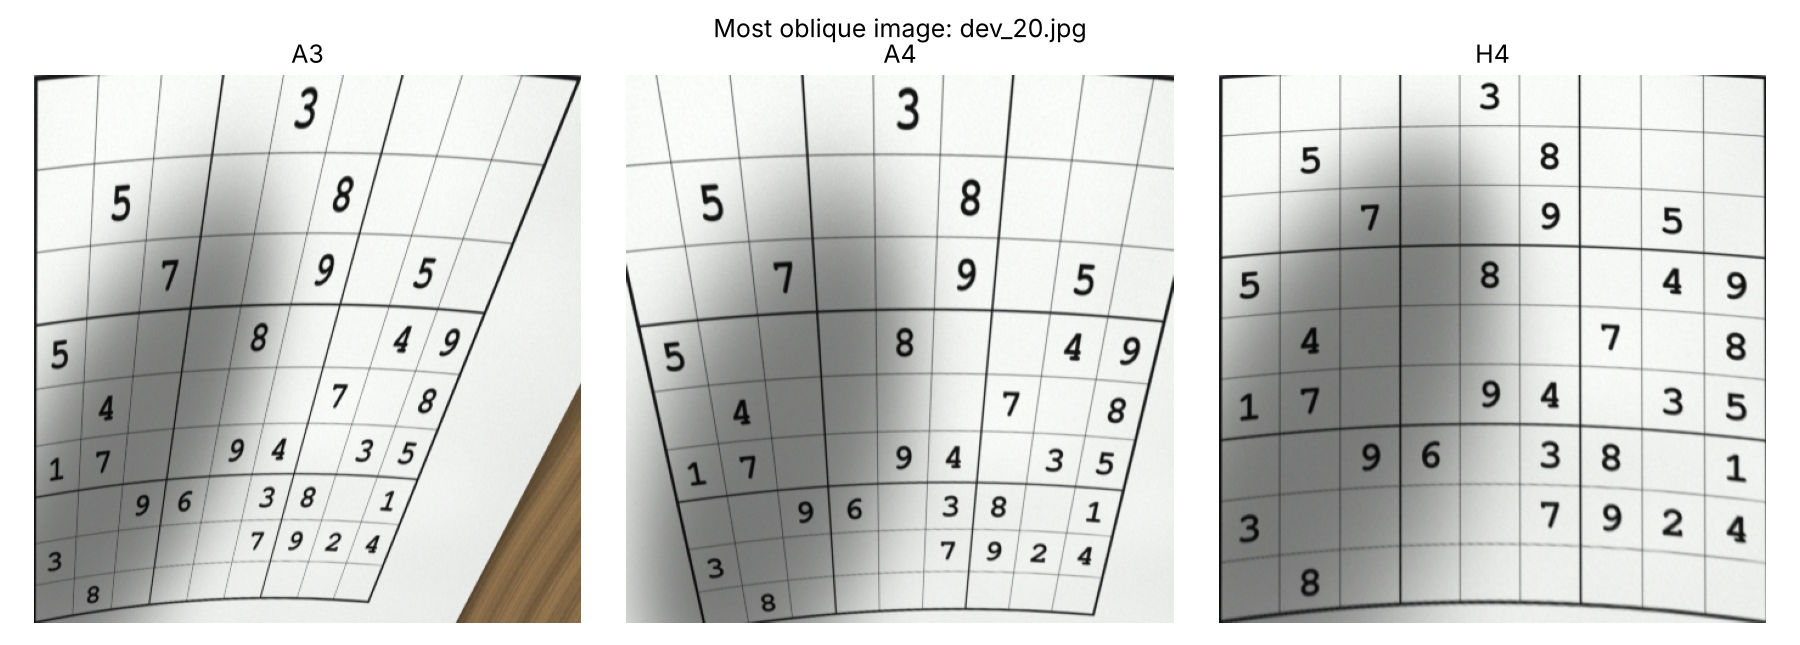
\includegraphics[width=\columnwidth]{devset/most_oblique.png}
\caption{A3, A4 and H4 rectifications of the most oblique development
image. \todo{replace with the most oblique personal image}.}
\label{fig:oblique}
\end{figure}

Both residuals grow steadily with obliqueness. The A3 error is about three to five
times the A4 residual, because A3 puts the whole misfit on one corner. With
H4 the grid lines stay within about 1\,px of their ideal positions at every
angle; the single exception (6.2\,px) is an image with a curled page, which
no $3\times3$ transformation can flatten. With the affine models the lines
are already several pixels off at a ratio of 1.05, and recognition breaks
down once the ratio exceeds about 1.2.

\textbf{Conclusion.} An affine model is an acceptable approximation only for
near-frontal views: up to an obliqueness of about 1.07 A4 still gave every
cell correctly, and up to about 1.18 it lost at most a few cells. A3 is
worse than A4 at small angles because its error is concentrated at one
corner. This agrees with the weak-perspective camera model. Perspective
projection divides by the depth $Z$; when the depth variation $\Delta Z$
across the object is small compared with its mean distance $\bar Z$, all
points are divided by nearly the same number and the projection of a plane
becomes affine. For a page of side $s$ tilted by $\theta$ at distance
$\bar Z$, $\Delta Z = s\sin\theta$, and the far side appears shorter than
the near side by the factor
$(\bar Z + \tfrac{1}{2}\Delta Z)/(\bar Z - \tfrac{1}{2}\Delta Z)$, which is
the obliqueness measured here. A phone held 30\,cm above a 15\,cm puzzle
violates $\Delta Z \ll \bar Z$ as soon as the page is tilted noticeably, so
a homography is required. \todo{confirm or adjust these limits with the
personal measurements}.

\section{Recognition}
\textbf{Cells and margin.} The H4 image is divided into 81 equal
$50\times50$ cells. Each cell has an inner margin of 7\,px (14\,\%) on every
side. The margin was chosen from measurements on the development set:
printed digits lie between 11 and 40\,px inside a cell, while grid lines
occupy only the first few pixels next to the cell boundary, so 7\,px
separates the two.

\textbf{Empty-cell criterion.} The rectified image is binarised as in
Stage~1 and split into connected components. A cell is filled when a
component that is smaller than a cell and at least 30\,\% of the cell height
has its centre inside the inner region of that cell. All other cells are
empty and are never passed to the OCR engine. Grid lines are either larger
than a cell or centred in the margin. Using the component instead of a hard
crop keeps a digit complete when the rectification is a few pixels off; with
a hard crop such digits touched the crop border and were lost.

\textbf{OCR configuration.} Tesseract~5 is used through
\texttt{pytesseract} with \texttt{--psm 10} (single character) and the
whitelist \texttt{123456789}. Table~\ref{tab:ocr} compares the page
segmentation modes. Modes 10 and 7 are best; modes 6, 8 and 13 are clearly
worse on isolated digits.

\textbf{Cell preparation.} The digit mask is drawn in black on a white
square whose side is 2.5 times the digit height, and resized to
$40\times40$\,px. This removes line remnants, centres the digit and gives
Tesseract the white border it needs. Feeding the raw grey cell instead
lowers cell accuracy from 0.994 to 0.943. Larger pictures were worse: at
$96\times96$ Tesseract returned an empty string for about one digit in ten.
Even with preparation, mode 10 occasionally returns nothing for a clear
digit but almost never returns a wrong one. Since the cell is already known
to be filled, an empty answer is retried with a padding of 2.0 and 3.0 and
finally with mode 13.

\begin{table}[t]
\caption{OCR variants (development set, cell accuracy)}
\label{tab:ocr}
\centering
\begin{tabular}{lr}
\toprule
Variant & Accuracy\\
\midrule
Prepared, psm 10 with retries (final) & 1.000\\
Prepared, psm 10 & 0.994\\
Prepared, psm 10, no whitelist & 0.995\\
Prepared, psm 7 & 0.994\\
Prepared, psm 13 & 0.931\\
Prepared, psm 8 & 0.928\\
Prepared, psm 6 & 0.915\\
Raw cells, psm 10 & 0.943\\
\bottomrule
\end{tabular}
\end{table}

\textbf{Confusions.} The final configuration makes no error on the
development set. \todo{list the most frequent confusions on the personal
dataset from \texttt{tools/ocr\_study.py}, with example crops from
\texttt{figures/personal/confusions/}}.

\section{Results}
Table~\ref{tab:results} gives the metrics of Section~7 of the assignment,
computed with \texttt{tools/evaluate.py}.

\begin{table}[t]
\caption{Results by condition}
\label{tab:results}
\centering
\begin{tabular}{lrrrrr}
\toprule
Group & $n$ & Corner (\%) & Cells & Empty F1 & Exact\\
\midrule
\multicolumn{6}{l}{\emph{Development set}}\\
All & 20 & 0.28 & 1.000 & 1.000 & 1.00\\
C1  & 5  & 0.27 & 1.000 & 1.000 & 1.00\\
C2  & 9  & 0.27 & 1.000 & 1.000 & 1.00\\
C3  & 4  & 0.31 & 1.000 & 1.000 & 1.00\\
C4  & 6  & 0.27 & 1.000 & 1.000 & 1.00\\
C5  & 6  & 0.31 & 1.000 & 1.000 & 1.00\\
\midrule
\multicolumn{6}{l}{\emph{Personal dataset} \todo{fill in}}\\
All &  &  &  &  & \\
C1  &  &  &  &  & \\
C2  &  &  &  &  & \\
C3  &  &  &  &  & \\
C4  &  &  &  &  & \\
C5  &  &  &  &  & \\
\bottomrule
\end{tabular}
\end{table}

Robustness is 1.00 on the development set: every image was processed
without a crash in about 3\,s. The development images are synthetic, so
these numbers are an upper bound for real photographs.

\section{Failure Analysis}
\todo{At least four failure cases from the personal dataset. For each one:
the \texttt{\_harris.png} or \texttt{\_debug.png} image, which stage failed
and why.} Two cases can be taken from the experiments above:

\emph{Affine rectification of an oblique view} (Fig.~\ref{fig:oblique}). The
failing stage is rectification: A3 and A4 leave converging grid lines, the
digits fall into the wrong cells and cell accuracy drops to 0.54.

\emph{Curled page} (development image 20). The corners are correct (0.24\,\%)
but the grid lines deviate by 6.2\,px after H4, because a curved surface is
not a plane. The cells were still read correctly only because the digit
components are assigned by their centre.

\section{Conclusion and Limitations}
The pipeline finds the puzzle from the structure of the grid itself (one
component with 81 holes) and takes the corners from the Harris detector. A
homography is necessary for anything but near-frontal views; the affine
models degrade in proportion to the ratio of opposite side lengths.

Limitations: the region rule needs closed cells and a grid that does not
touch other ink; a single homography cannot correct a curled page; a digit
that touches a grid line is merged with it and lost; and the fixed 85\,\%
ink threshold was tuned on synthetic images. \todo{adjust after the
personal dataset results}.

\end{document}
